\documentclass[letterpaper,12pt]{article}

\usepackage{ucs}
\usepackage[utf8x]{inputenc}
\usepackage{amsmath}
\usepackage{amsfonts}
\usepackage{amssymb}
\usepackage[margin=1in]{geometry}
\usepackage{graphicx}
\newcommand{\abs}[1]{\lvert #1\rvert}
\newcommand{\R}{\mathbb{R}}
\newcommand{\C}{\mathbb{C}}
\newcommand{\dotp}{\boldsymbol{\cdot}}

\title{Math 2580 Assignment \#4 Solutions\\University of Lethbridge, Spring 2016}
\author{Sean Fitzpatrick}
\begin{document}
 \maketitle


\begin{enumerate}
 \item Evaluate the integeral below, where $D=\{(x,y) | x^2+y^2\leq 1\}$ is the unit disc. Explain your result.
\[
 \iint_D (x^3e^{x^2}+y^{1/3}\sin(y^4)+3)\,dA.
\]
Hint: as regions go, the unit disc is about as symmetric as they get.

\bigskip

Of the three terms in the integrand, we note that the first is an odd function of $x$, and the second is an odd function of $y$. Since the region $D$ is symmetric with respect to both $x$ and $y$, neither of these terms contribute to the integral. Thus, 
\[
 \iint_D (x^3e^{x^2}+y^{1/3}\sin(y^4)+3)\,dA = \iint_D 3\,dA = 3\pi,
\]
since the region $D$ is a disc, and thus has area $\pi(1)^2=\pi$.

 \item The integral below expresses the integral of a function $f$ over a region $D$ as a sum of two iterated integrals. Sketch the region of integration, and express the integral as a single iterated integral with the order of integration reversed:
\[
 \iint_D f(x,y)\,dA = \int_0^1\int_1^{x^2+1}f(x,y)\,dy\,dx + \int_1^3\int_1^{\frac{1}{4}(x-3)^2+1}f(x,y)\,dy\,dx.
\]

The region is sketched below:
\begin{center}
 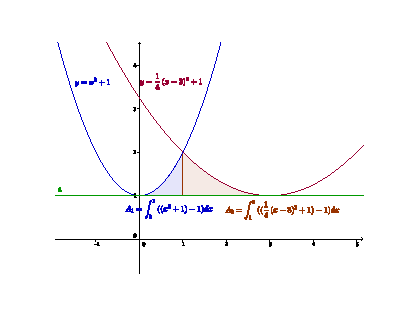
\includegraphics[width=0.7\textwidth]{WS4-1c}
\end{center}
The curves intersect at the point $(1,2)$, so we have $1\leq y\leq 2$. The equation $y=x^2+1$ can be written as $x=\pm \sqrt{y-1}$; since our region is bounded by the right half of this parabola, we have $x=\sqrt{y-1}$.  Similarly, $y=\frac{1}{4}(x-3)^2+1$ gives us $(x-3)^2 = 4(y-1)$, so $x=3\pm 2\sqrt{y-1}$. Since our region is bounded by the left half of this parabola, we take $x=3-2\sqrt{y-1}$. Thus, for each $y\in [1,2]$, we have $\sqrt{y-1}\leq x\leq 3-2\sqrt{y-1}$. It follows that
\begin{align*}
 \iint_D f(x,y)\,dA &= \int_0^1\int_1^{x^2+1}f(x,y)\,dy\,dx + \int_1^3\int_1^{\frac{1}{4}(x-3)^2+1}f(x,y)\,dy\,dx\\
& = \int_1^2\int_{\sqrt{y-1}}^{3-2\sqrt{y-1}}f(x,y)\,dx\,dy.
\end{align*}

 \item Prove that $\displaystyle 2\int_a^b\int_x^b f(x)f(y)\,dy\,dx = \left(\int_a^b f(x)\,dx\right)^2$.

{\em Hint:} Notice that $\left(\int_a^b f(x)\,dx\right)^2 = \iint_{[a,b]\times [a,b]}f(x)f(y)\,dA$.

\bigskip

We first establish the hint: since $f(x)$ is constand with respect to $y$, we have
\begin{align*}
 \int_a^b\int_a^b f(x)f(y)\,dy\,dx &= \int_a^b f(x) \left(\int_a^b f(y)\,dy\right)\,dx\\
& = \int_a^b f(y)\,dy \int_a^bf(x)\,dx \\
& = \left(\int_a^b f(x)\,dx\right)^2.
\end{align*}
(In the last two equalities we used the fact that $\int_a^b f(y)\,dy$ is a constant, and therefore can be taken out of the integral, followed by the fact that we can use whatever letter we want for the integration variable.)

On the other hand, we can write
\begin{align}
 \int_a^b\int_a^b f(x)f(y)\,dy\,dx &= \int_a^b \left(\int_a^x f(x)f(y)\,dx +\int_x^b f(x)f(y)\,dx \right)\,dy \nonumber\\
 & = \int_a^b\int_a^x f(x)f(y)\,dy\,dx + \int_a^b\int_x^b f(x)f(y)\,dy\,dx.\label{a}
\end{align}
The above equality can be viewed as a consequence of the property $\int_a^b f(x)\,dx = \int_a^c f(x)\,dx + \int_c^b f(x)\,dx$ of single integrals, or in terms of properties of double integrals, as follows: Let $R=[a,b]\times [a,b]$ denote the given rectangle, and note that we can write $R=D_1\cup D_2$, where $D_1$ is the triangle lying above the line $y=x$ in $R$, and $D_2$ is the triangle lying below the line $y=x$ in $R$.

The region $D_1$ is given by $x\leq y\leq b$, where $a\leq x\leq b$, and this corresponds to the second integral above. The region $D_2$ is given by $a\leq y\leq x$, where $a\leq x\leq b$, and this is the first integral above. However, we can also write $D_2$ as the Type 2 region given by $y\leq x\leq b$, where $a\leq y\leq b$. Thus,
\begin{align*}
 \iint_{D_2}f(x)f(y)\,dA &= \int_a^b\int_a^x f(x)f(y)\,dy\,dx \\
& = \int_a^b\int_y^b f(x)f(y)\,dx\,dy \\
& = \int_a^b\int_x^b f(y)f(x)\,dy\,dx,
\end{align*}
 where in the last equality we've used the fact that we're free to rename the variables (so $x$ has been renamed $y$, and vice versa). Substituting this result into \eqref{a} above, we obtain our result.
\pagebreak
 \item Prove the following Mean Value Theorem for double integrals: suppose $D\subseteq \R^2$ is an elementary region (Type 1 or Type 2), and that $f:D\to \R$ is continuous. Then there exists a point $(x_0,y_0)\in D$ such that 
\[
 \iint_Df(x,y)\,dA = f(x_0,y_0)A(D),
\]
where $A(D)$ denotes the area of $D$. \\
(Note that $\frac{1}{A(D)}\iint_D f(x,y)\,dA$ gives the average value of $f$ on $D$.)

You may use the following facts in your proof:
\begin{itemize}
 \item The Extreme Value Theorem holds in $\R^2$: if $D\subseteq \R^2$ is closed and bounded\footnote{A subset of $\R^n$ is {\em closed} if it contains its boundary. It is {\em bounded} if it can be contained within a disk of sufficiently large radius: it doesn't go off to infinity in any direction.} and $f:D\to\R$ is continuous, then there exist $m,M\in\R$ such that $m\leq f(x,y)\leq M$ for all $(x,y)\in D$; moreover, there exist points $(x_1,y_1), (x_2,y_2)\in D$ such that $f(x_1,y_1)=m$ and $f(x_2,y_2)=M$. (That is, $f$ attains its minimum and maximum values on $D$.)

 \item The Intermediate Value Theorem holds in $\R^2$: Suppose $D\subseteq \R^2$ is connected\footnote{A subset $D$ of $\R^2$ is {\em connected} if it is impossible to find two non-intersecting disks that both contain part of $D$. In other words, $D$ cannot be split into two pieces that do not touch. Note that in particular, every elementary region is connected.} and $f:D\to \R$ is continuous. Then if $f(x_1,y_1)=a$ for some $(x_1,y_1)\in D$ and $f(x_2,y_2)=b$ for some $(x_2,y_2)\in D$, and $c$ is any real number between $a$ and $b$, then there exists some point $(x_0,y_0)\in D$ such that $f(x_0,y_0)=c$.
\end{itemize}

\bigskip

The proof is as follows: Since $f$ is continuous on $D$, there exist points $(x_1,y_1), (x_2,y_2)\in D$ such that
\[
 f(x_1,y_1)=m\leq f(x,y)\leq M=f(x_2,y_2)
\]
for all $(x,y)\in D$, by the Extreme Value Theorem. It follows that
\[
 mA(D) = \iint_D m \,dA \leq \iint_D f(x,y)\,dA \leq \iint_D M\,dA = MA(D),
\]
where $A(D) =\iint_D\,dA$ is the area of $D$. Since $A(D)>0$, we can divide the above inequality by $A(D)$, giving us
\[
 f(x_1,x_2) = m\leq \frac{1}{A(D)}\iint_D f(x,y)\,dA \leq M = f(x_2,y_2)
\]
We are told that the Intermediate Value Theorem holds for the region $D$, so the above inequality implies that there must exist some point $(x_0,y_0)\in D$ such that
\[
 f(x_0,y_0) = \frac{1}{A(D)}\iint_D f(x,y)\,dA,
\]
completing the proof.



\end{enumerate}



\end{document}
 
